\documentclass[12pt]{article}
\usepackage[margin=1in]{geometry}
\usepackage{enumerate}
\usepackage{graphicx}


\title{EECS 314 - Project Report}
\author{Haley Eisenshtadt, Jason Kuster, Ian Lavelle, Joseph Satterfield, James Wright}

\begin{document}
	\maketitle
	\section{Problem Statement}
	While learning MIPS in EECS 314, our group noticed a lack of fun, interactive tools to make learning MIPS easier. There are helpful demonstrations in the textbook and you can always open up QtSpim and play around, but there wasn't anything particularly graphical and interactive to help people learn MIPS. Our group wanted to put together an Android app to make the process of learning MIPS easier. The tool we settled on to build this was Unity, a cross-platform game engine which several of us had used before which made game development easy.
	\section{Major Challenges}
	There were a couple of challenges we ran up against while developing this set of games.
	% Put some major challenges we ran up against here. Format is \item <PUT TEXT HERE>
	\begin{enumerate}
		\item User interface design in Unity. Unity recently switched to using a new user interface system, and setting up all of the click interactions within MIPS simulator was non-trivial in the new system, requiring nesting function definitions within functions. Also, setting up a system to let the various operands know what types they can accept was a challenge as it essentially involved keeping lists of which slots would accept various operand types, and then forcing them to correctly highlight.
		\item In the original game Bejeweled (and its clone Candy Crush), the goal is to simply match lines of identical pieces, regardless of order. Our initial thought was to just make Bejeweled and then change the sprites to make it MIPS themed, but becasue MIPS relies on a specific order of different items, we were forced to rethink large sections of code. Now, there are specific OP pieces which tell the game how many pieces to check and in what order the different inputs should be.
	\end{enumerate}
	\section{Key Components}
	Our project has three key components which come together to make the MIPS learning process easier. We have the MIPS Simulator, which is a graphical MIPS simulator in the style of ALICE for Java, we have MIPS Bejeweled, a twist on the classic Bejeweled game which helps teach people how MIPS instructions work, and we have the Pipeline Bakery which presents the MIPS pipeline in a fun, graphical way.
	\subsection{MIPS Simulator}
	The MIPS Simulator allows the user to use an intuitive user interface to create a sequence of instructions and view the results of those instructions. You start by adding new instructions via the instructions panel and then filling in the operands using the various operand kind panels. Operands will only let you place themselves in valid instruction positions to help reduce the amount of error that can occur.
	\subsection{MIPS Bejeweled}
	MIPS Bejeweled takes the classic bejeweled game and adds the twist of only completing rows when those rows create a valid MIPS instruction. In order to make this work we needed to remove the requirement in Bejeweled of reversing a move if it doesn't make a valid combination, because with the added complexity of MIPS instructions the game was impossible to play. We feel that this is an acceptable compromise in the name of usability. We also changed out the typical falling physics of classic Bejeweled for a swapping mechanism that encourages the player to think ahead.
	\subsection{Pipeline Bakery}
	Pipeline Bakery is designed to be a simple, entertaining introduction to the MIPS pipeline. The game includes a tutorial which guides the player through the different stages of an instruction, the construction of the MIPS pipeline, and the different pipeline hazards computer architects run into. The game portion of Pipeline Bakery is designed to quiz users on their knowledge of pipeline hazards. The game includes hardware hazards which are not found in the MIPS pipeline, but we wanted to illustrate all of the most common issues that computer architects run into when designing a pipeline. 
	\section{Integration}
	The integration of the three games was relatively simple. Each game was made seperately and then merged with GitHub into one folder. James went through and resolved any file conflicts in that arose from the merge. When together, each game takes place in what Unity calls a scene, including the main game-select screen. When the player selects a game to play, the scene of the desired game is loaded up, and the user plays it as normal. To go back, each game has another button that returns the user to the game-select screen.
	\section{User Interface}
	This project has three main UIs, one for each game, in addition to a main menu which is used to navigate to the individual projects. The MIPS simulator's UI was designed in order to remove many of the struggles of programming in MIPS. To start, you touch the instruction panel icon on the left, and click on an instruction to add it to the screen. Touch outside the panel to close it. Instructions can be moved around by tapping the icon to the left of the instruction name and then using the up and down arrows to move instructions. The center button lets you delete the selected instruction. To hide the line adjustment tools, tap anywhere away from them. Operands can be added by opening up the appropriate panels and tapping them. The appropriate locations will highlight in green - tap any one to replace the current value with whatever you selected. Tap the panel close button on the top left to exit out of operand placement mode. When you have placed all the operands, the code can be run using the run button, and a panel will show up with the results of the instructions.
	\subsection{MIPS Simulator}
	\subsection{MIPS Bejeweled}
	The UI for this was quite basic. Each gem has an input or an OP on it, and is colored according to what type it is. Blue is registers, yellow is a register with a shift, orange is an immediate value, red is an operation, and green is a jump address. The values on the pieces has no bearing on the game, but is just there as an example of what these values might look like in MIPS code. The first selected piece becomes larger than the others, indicating it has been selected and can be swapped with any adjacent piece.
	\subsection{Pipeline Bakery}
	The Pipeline Bakery UI is very straightforward. The tutorial is a touch-to-proceed format, and the game itself follows a similar control scheme. The donuts represent instruction stages. When a hazard appears, the donuts are highlighted red, and when the user resolves the hazard, the donuts are highlighted green. Instructions are displayed next to rows of donuts to give the user hazard type clues.
	\section{Snapshots}
	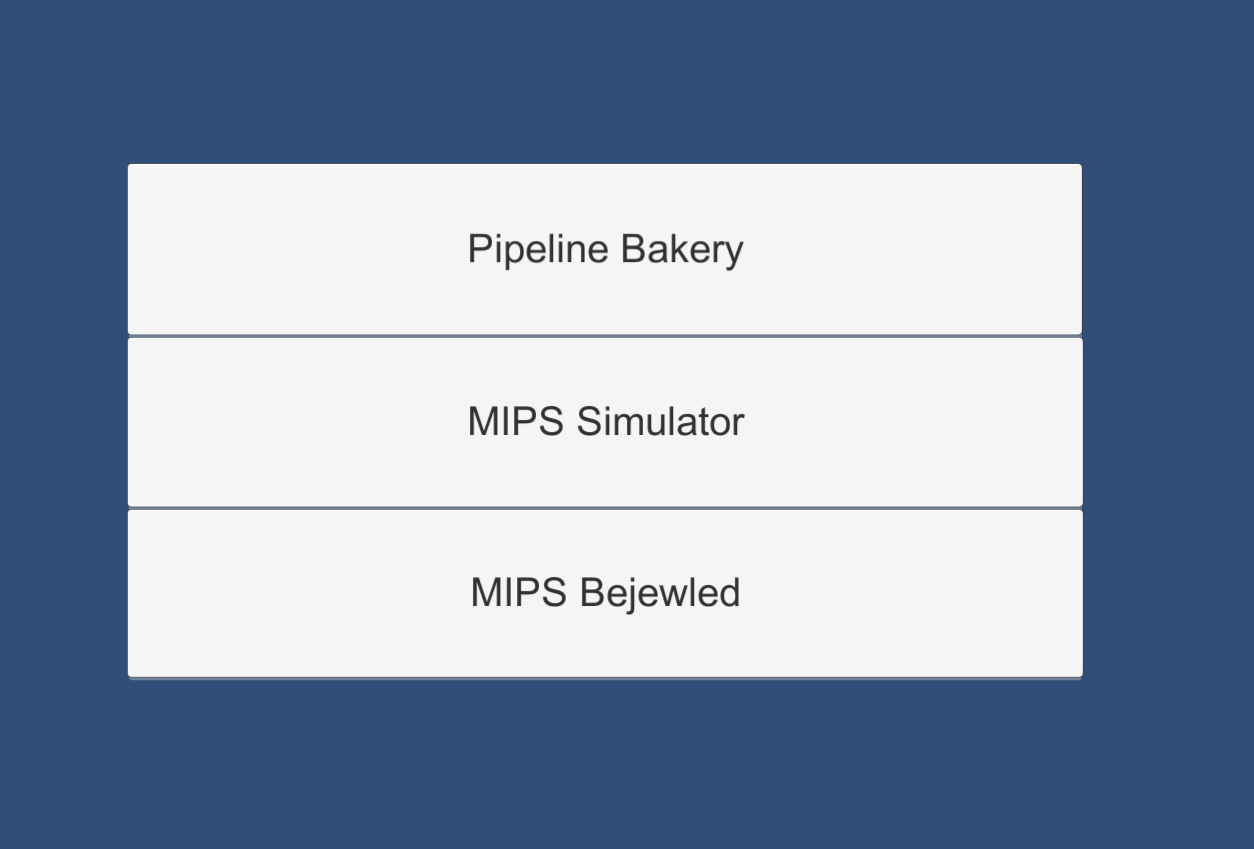
\includegraphics[height=8cm]{MainMenu.png}\\
	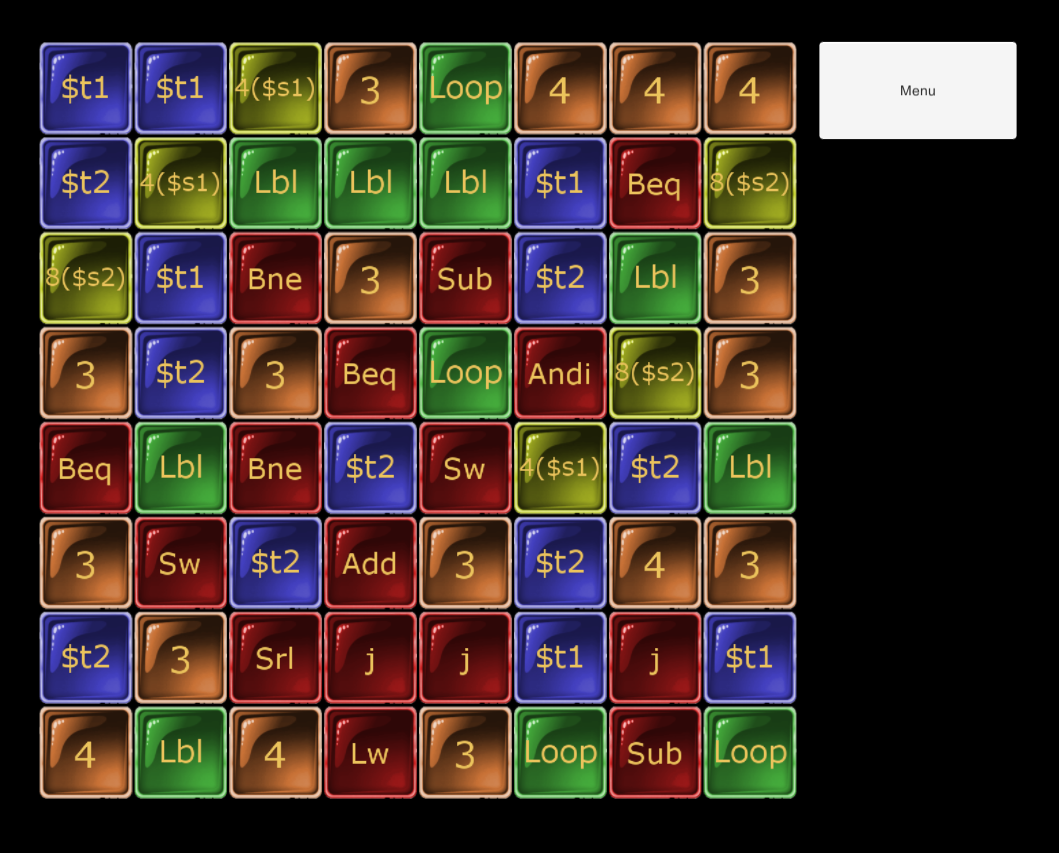
\includegraphics[height=6cm]{MIPSBejeweled.png}
	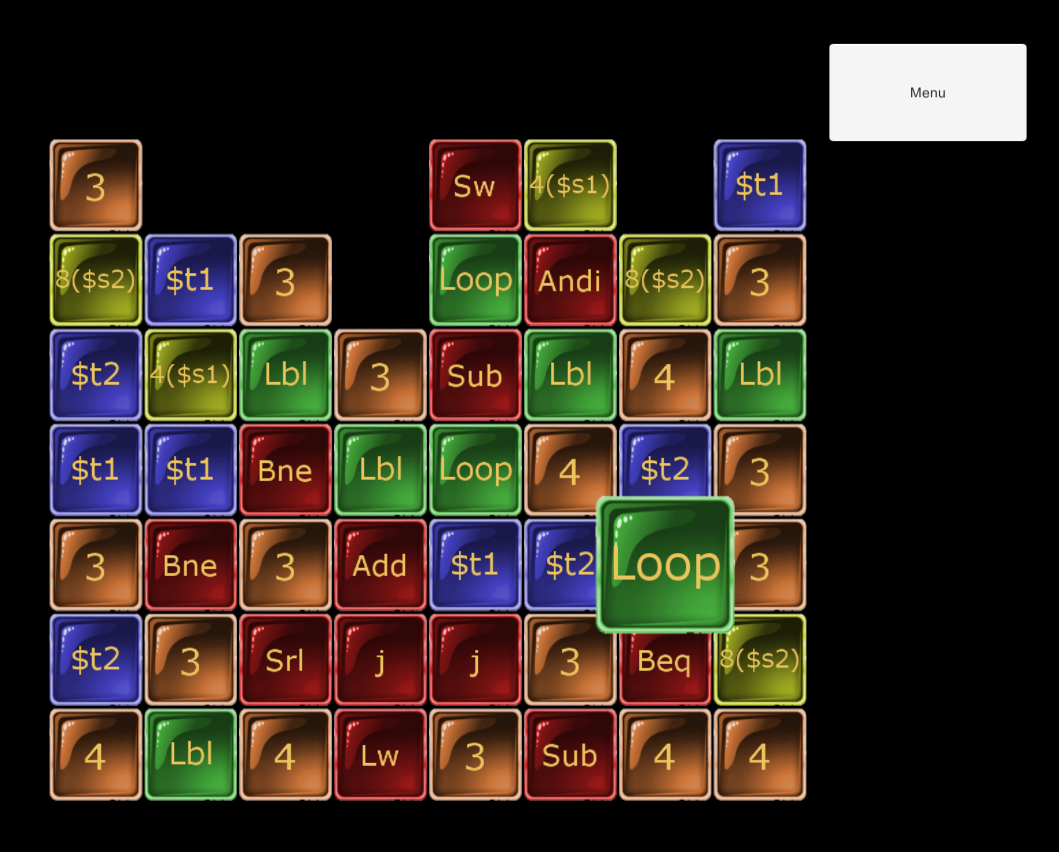
\includegraphics[height=6cm]{BejeweledHowTo.png}\\
	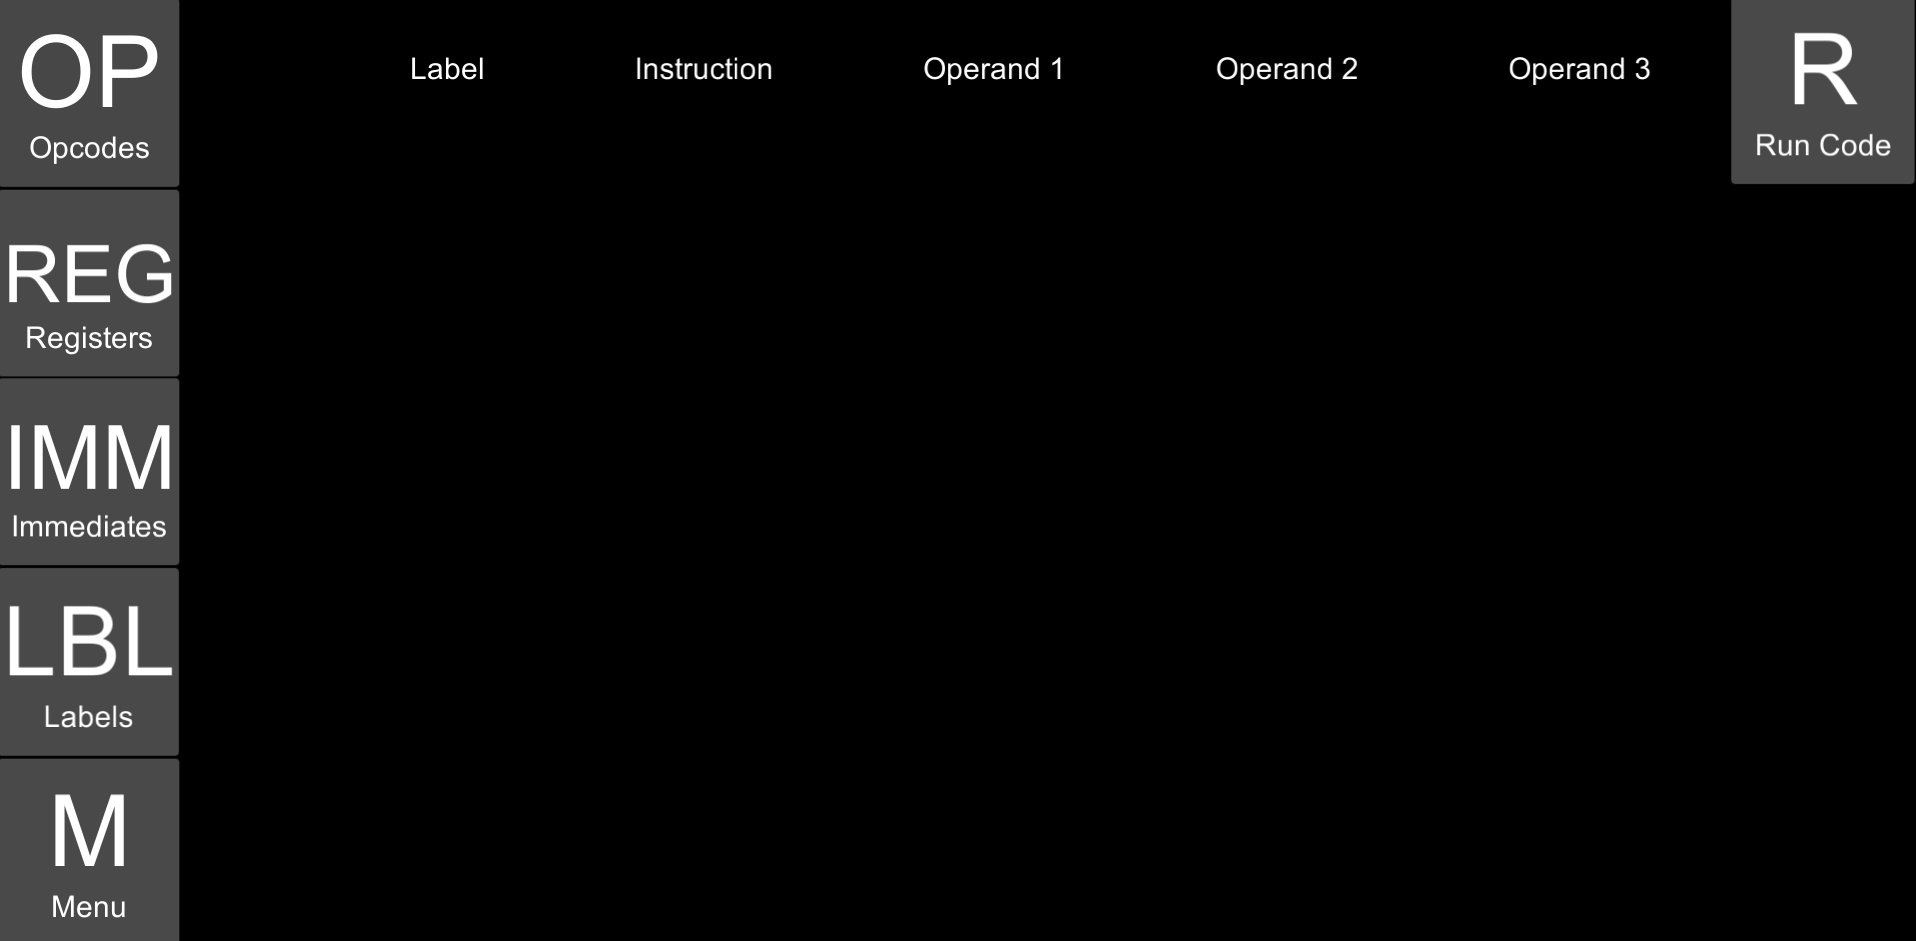
\includegraphics[height=4cm]{MIPSSimulatorStart.png}
	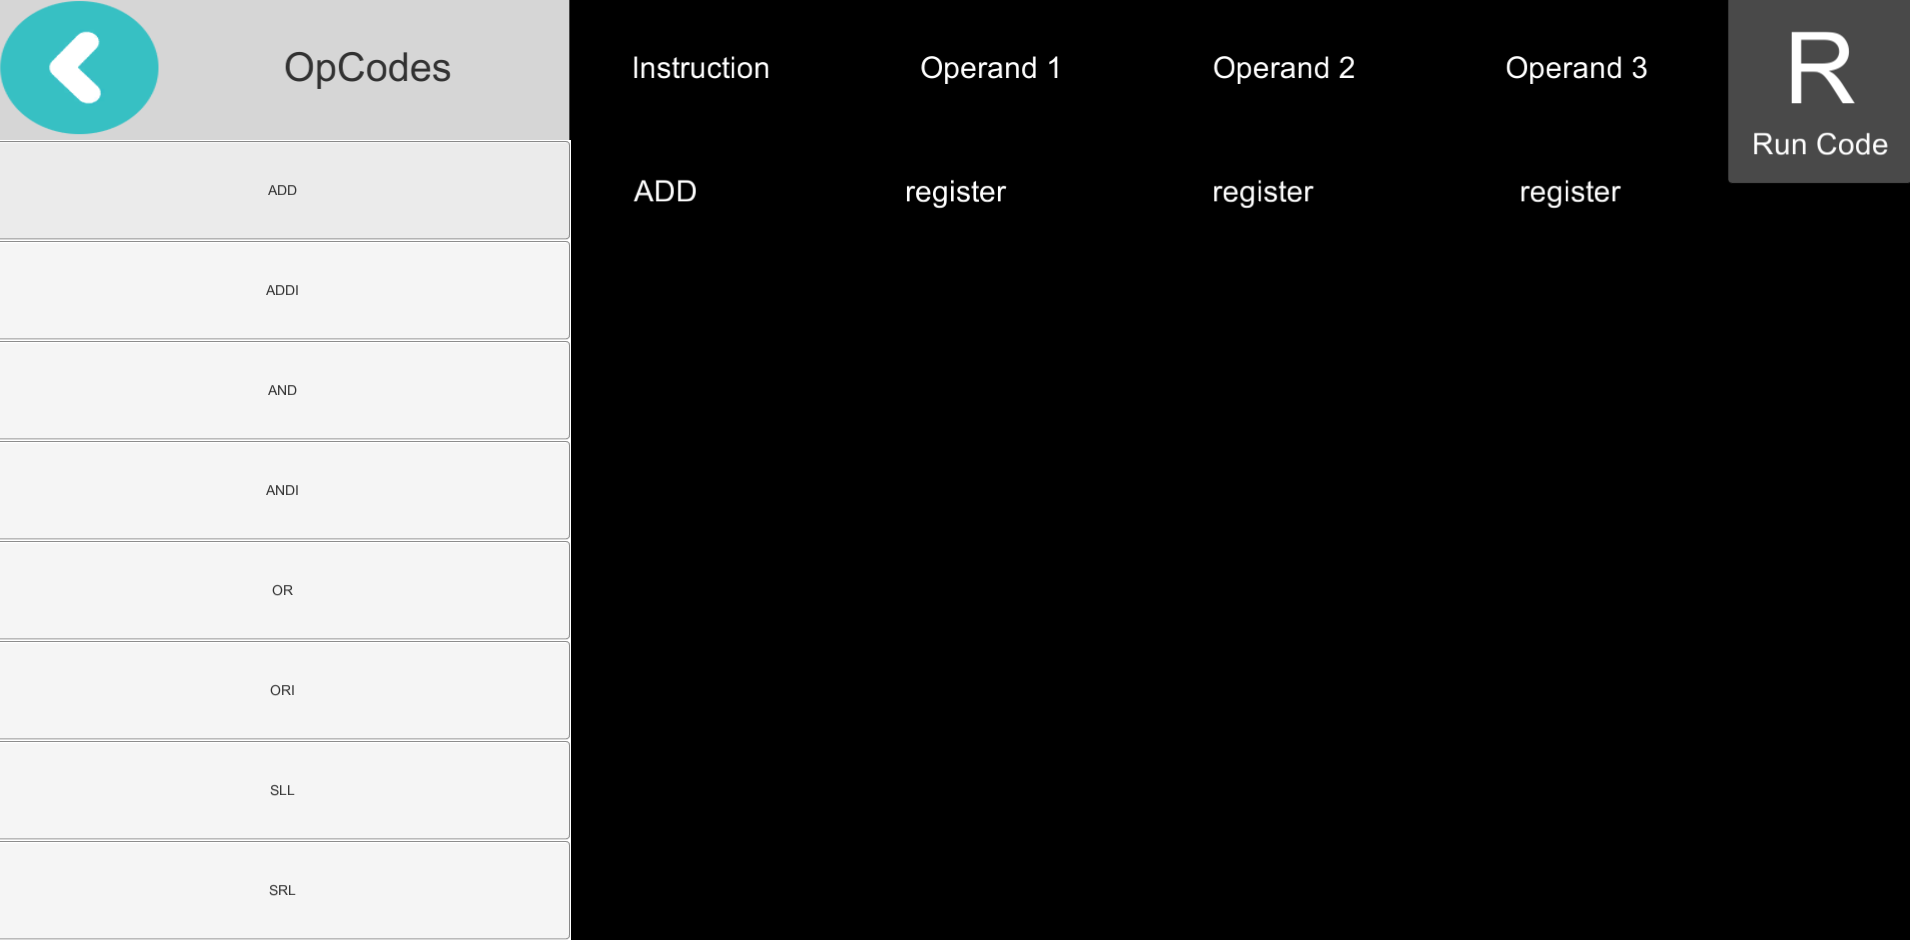
\includegraphics[height=4cm]{MIPSSimulatorProgress.png}\\
	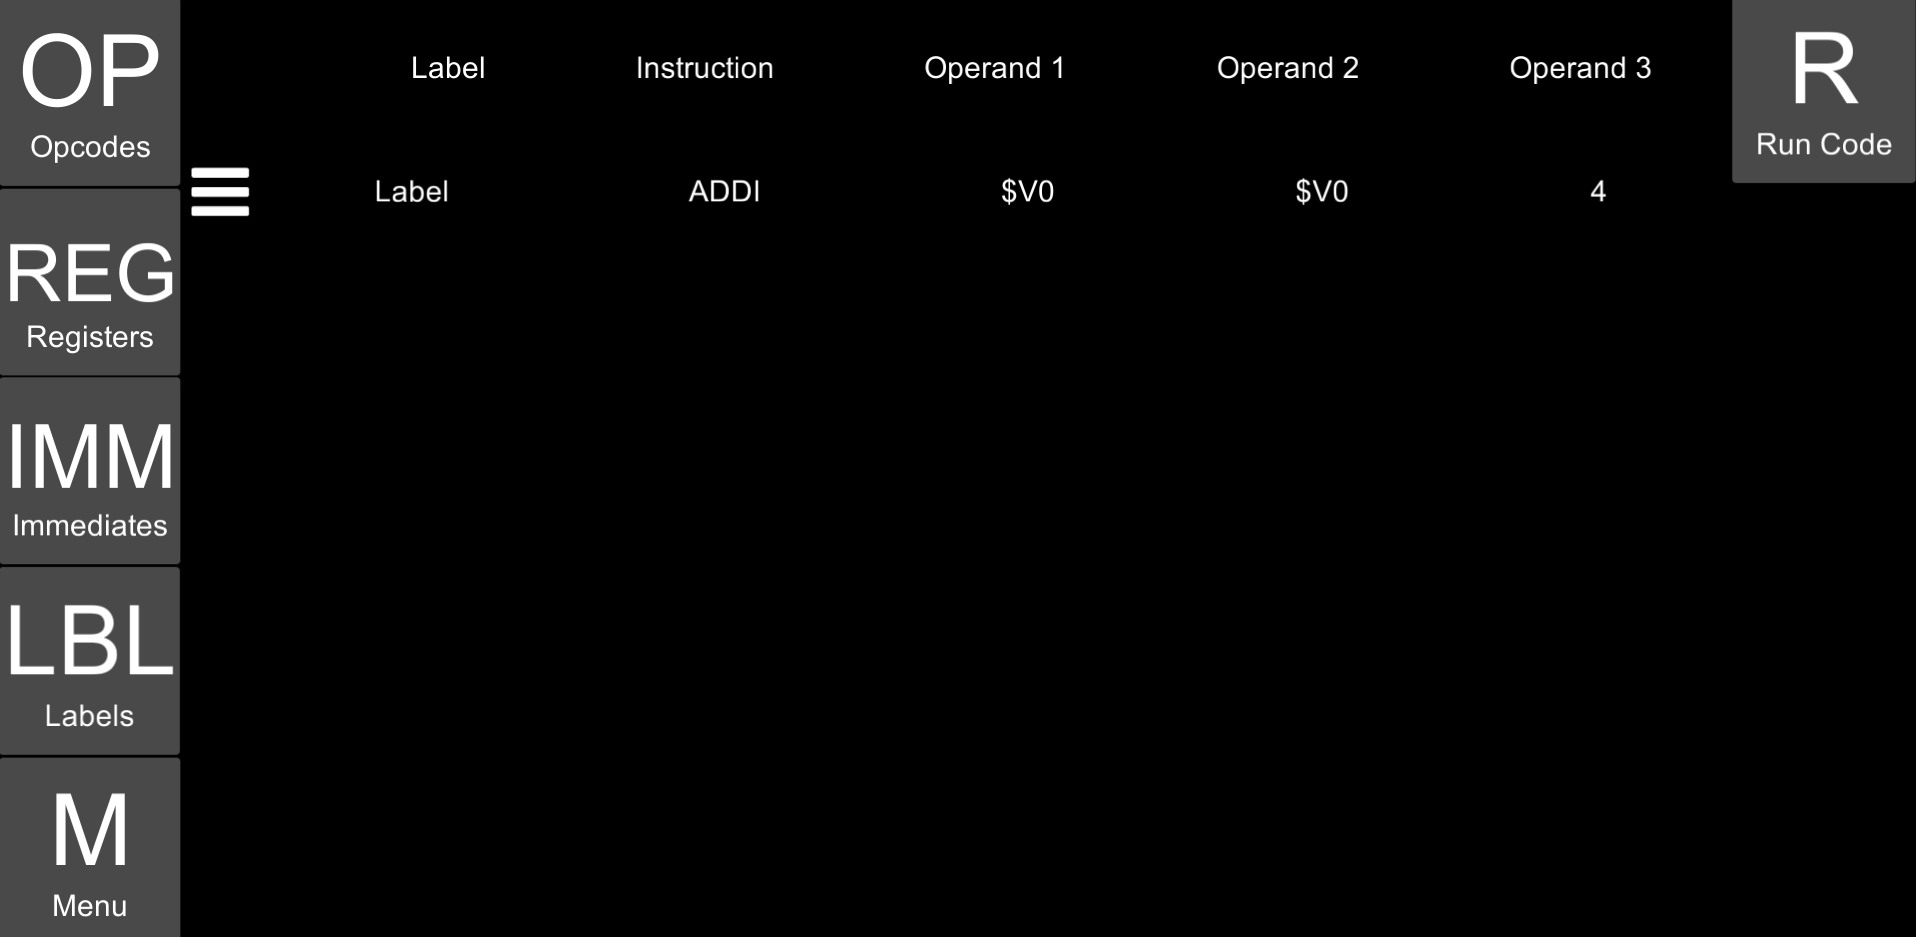
\includegraphics[height=4cm]{MIPSSimulatorReady.png}
	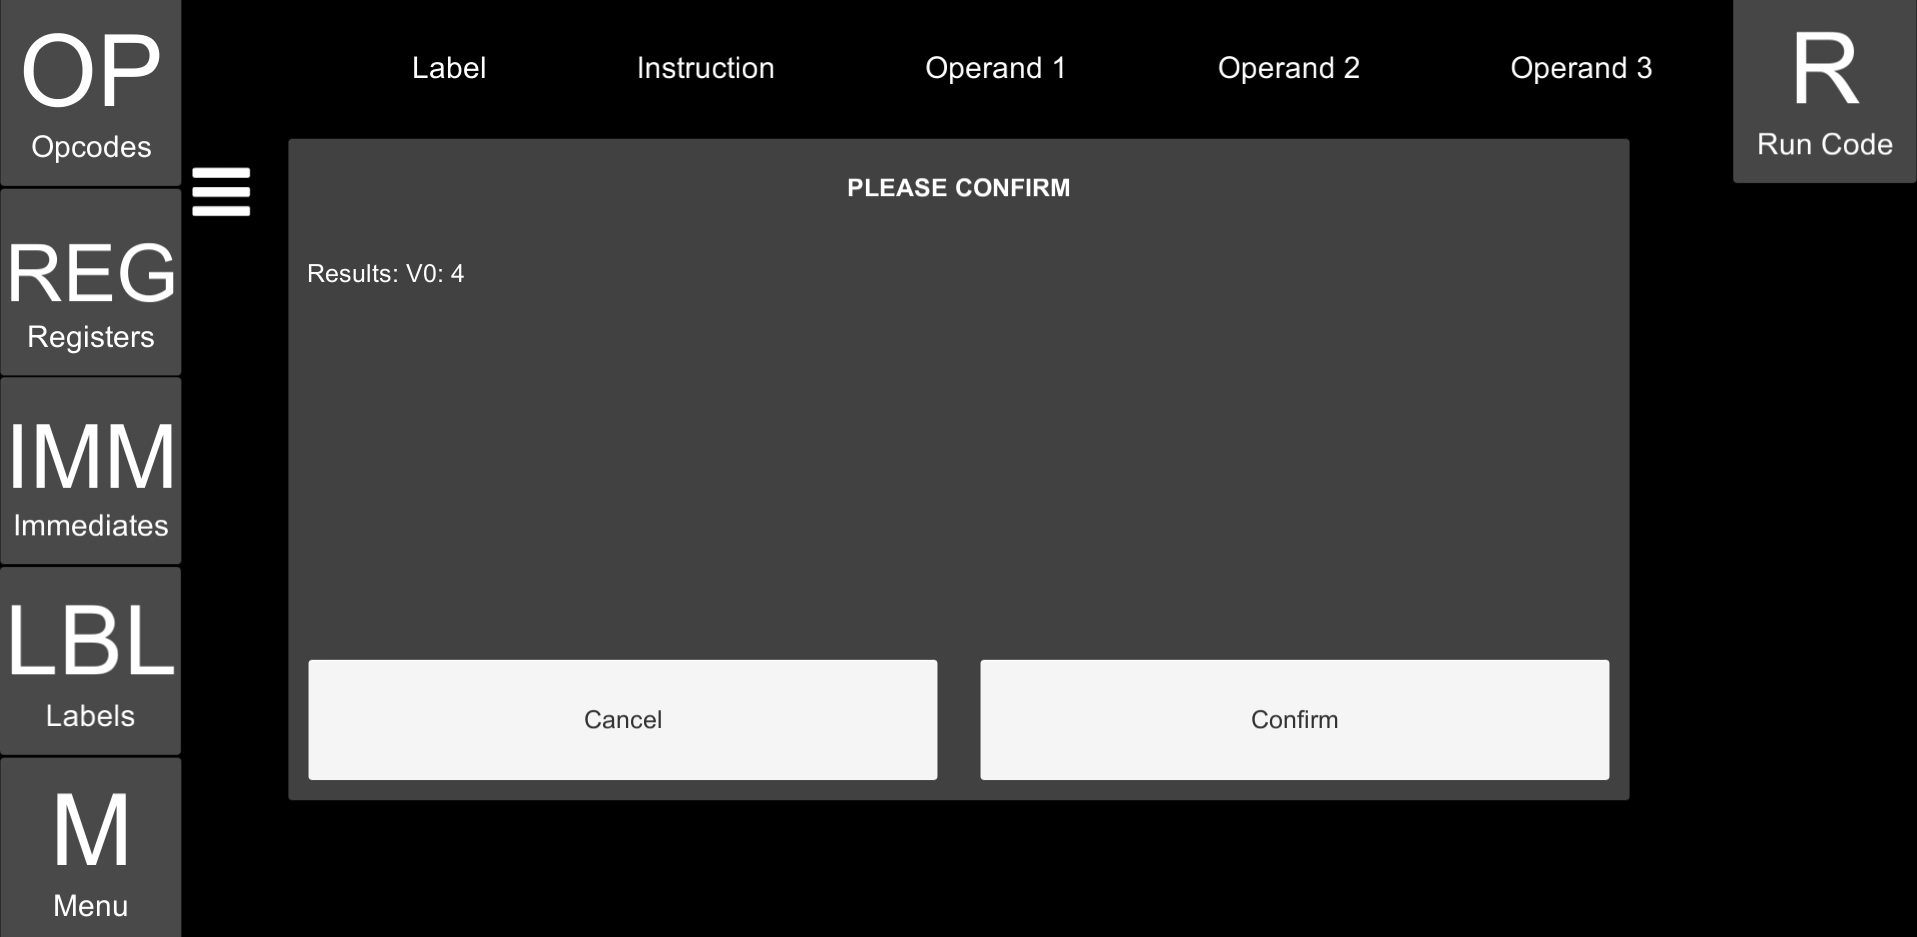
\includegraphics[height=4cm]{MIPSSimulatorRun.png}\\
	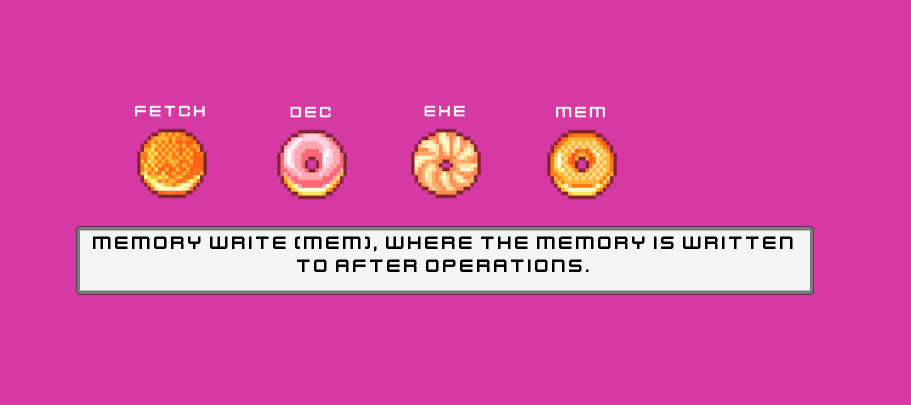
\includegraphics[height=4cm]{PipelineBakeryTut.png}
	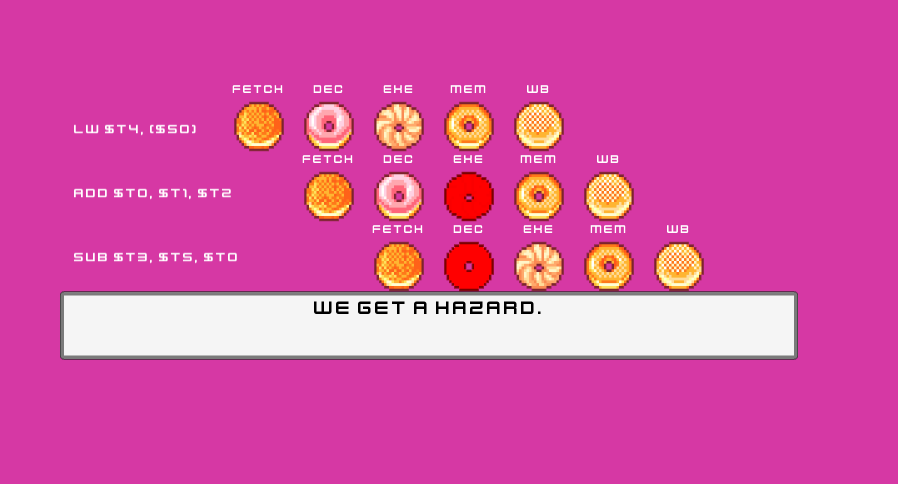
\includegraphics[height=4cm]{PipelineBakeryTut2.png}\\
	\section{Individual Contributions}
	\begin{itemize}
		\item Haley Eisenshtadt
		\subitem Pipeline Bakery Design/Implementation
		\item Jason Kuster
		\subitem Bejeweled Block Physics
		\subitem Project Report Lead/Compilation
		\item Ian Lavelle
		\subitem Bejeweled Base Implementation
		\subitem Bejeweled Instruction Logic
		\item Joe Satterfield
		\subitem MIPS Learner Simulator Back-End Implementer
		\item James Wright
		\subitem MIPS Learner User Interface Desgin and Implementer
	\end{itemize}
\end{document}
